\section{Redesign and Retuning}

The body-loaded simulations showed that the free-space-tuned dipole no longer remained well matched at the design operating frequency. Since the \(5~\mathrm{mm}\) case exhibited a clear downward shift of the matching minimum, it was selected for a first-order retuning study based on shortening the dipole length.

\subsection{Motivation for Retuning}

The tuned free-space dipole had good impedance matching at the target frequency,

\[
f_0 = 1.120~\mathrm{GHz},
\]

with

\[
S_{11}(1.120~\mathrm{GHz}) = -15.48433~\mathrm{dB}.
\]

However, when the same dipole was placed \(5~\mathrm{mm}\) above the body model, the matching minimum shifted downward to

\[
f_{\min} = 0.9792~\mathrm{GHz},
\]

and the return loss at the target frequency degraded to

\[
S_{11}(1.120~\mathrm{GHz}) = -5.903831~\mathrm{dB}.
\]

This indicates that the \(122.0~\mathrm{mm}\) dipole became electrically too long in the presence of the nearby high-permittivity body model. Therefore, the first retuning strategy was to shorten the dipole length.

\subsection{First-Order Length Estimate}

A first-order retuning estimate was obtained by using the approximate inverse relationship between resonant frequency and dipole length,

\[
f_r \propto \frac{1}{L}.
\]

The estimated new length was calculated as

\[
L_{\mathrm{new}}
=
L_{\mathrm{old}}
\frac{f_r}{f_0},
\]

where \(L_{\mathrm{old}}\) is the original tuned free-space dipole length, \(f_r\) is the observed matching-minimum frequency near the body, and \(f_0\) is the desired operating frequency.

For the \(5~\mathrm{mm}\) body-separation case,

\[
L_{\mathrm{old}} = 122.0~\mathrm{mm},
\]

\[
f_r = 0.9792~\mathrm{GHz},
\]

and

\[
f_0 = 1.120~\mathrm{GHz}.
\]

Therefore,

\[
L_{\mathrm{new}}
=
122.0
\frac{0.9792}{1.120}
=
106.66~\mathrm{mm}.
\]

The Python verification of this body-loaded retuning estimate is included in Appendix~\ref{app:python-utility-calculations}, Listing~\ref{lst:wearable-verification}.

Based on this first-order estimate, the retuned CST dipole length was selected as

\[
L = 106.6~\mathrm{mm}.
\]

With the \(2~\mathrm{mm}\) center feed gap, the corresponding arm length was

\[
L_{\mathrm{arm}}
=
\frac{106.6-2.0}{2}
=
52.3~\mathrm{mm}.
\]

Thus, the retuned CST geometry used the right and left arm coordinates listed in Table~\ref{tab:retuned-l106p6-geometry}.

\begin{table}[htbp]
\centering
\caption{Retuned dipole geometry for \(L=106.6~\mathrm{mm}\) and \(2~\mathrm{mm}\) feed gap.}
\label{tab:retuned-l106p6-geometry}
\begin{tabular}{lc}
\hline
\textbf{Parameter} & \textbf{Value} \\
\hline
Total dipole length & \(106.6~\mathrm{mm}\) \\
Feed gap & \(2.0~\mathrm{mm}\) \\
Wire radius & \(0.905~\mathrm{mm}\) \\
Each arm length & \(52.3~\mathrm{mm}\) \\
Right arm \(x\)-range & \(1.0~\mathrm{mm}\) to \(53.3~\mathrm{mm}\) \\
Left arm \(x\)-range & \(-53.3~\mathrm{mm}\) to \(-1.0~\mathrm{mm}\) \\
Port reference impedance & \(50~\Omega\) \\
\hline
\end{tabular}
\end{table}

\subsection{Retuned Result for \(L=106.6~\mathrm{mm}\)}

The \(L=106.6~\mathrm{mm}\) retuned dipole was simulated above the same \(5~\mathrm{mm}\) body model. The CST result showed that the matching minimum moved closer to the target frequency. The minimum occurred at

\[
f_{\min} = 1.0928~\mathrm{GHz},
\]

with

\[
S_{11,\min} = -8.152857~\mathrm{dB}.
\]

At the target frequency,

\[
f_0 = 1.120~\mathrm{GHz},
\]

the return loss improved to

\[
S_{11}(1.120~\mathrm{GHz}) = -8.000936~\mathrm{dB}.
\]

\begin{table}[htbp]
\centering
\caption{Retuned result for the \(5~\mathrm{mm}\) body-separation case using \(L=106.6~\mathrm{mm}\).}
\label{tab:retuned-l106p6-result}
\begin{tabular}{lc}
\hline
\textbf{Quantity} & \textbf{Value} \\
\hline
Antenna-body separation & \(5~\mathrm{mm}\) \\
Retuned dipole length & \(106.6~\mathrm{mm}\) \\
Feed gap & \(2.0~\mathrm{mm}\) \\
Minimum-\(S_{11}\) frequency & \(1.0928~\mathrm{GHz}\) \\
Minimum \(S_{11}\) & \(-8.152857~\mathrm{dB}\) \\
\(S_{11}\) at \(1.120~\mathrm{GHz}\) & \(-8.000936~\mathrm{dB}\) \\
\hline
\end{tabular}
\end{table}

Compared with the original \(5~\mathrm{mm}\) body case, the return loss at the target frequency improved from

\[
-5.903831~\mathrm{dB}
\]

to

\[
-8.000936~\mathrm{dB}.
\]

This confirms that shortening the antenna partially compensated for the downward detuning caused by the body model.

The return-loss response after shortening the dipole to \(106.6~\mathrm{mm}\) for the \(5~\mathrm{mm}\) body-separation case is shown in Figure~\ref{fig:retuned-l106p6-s11}.

\begin{figure}[htbp]
\centering
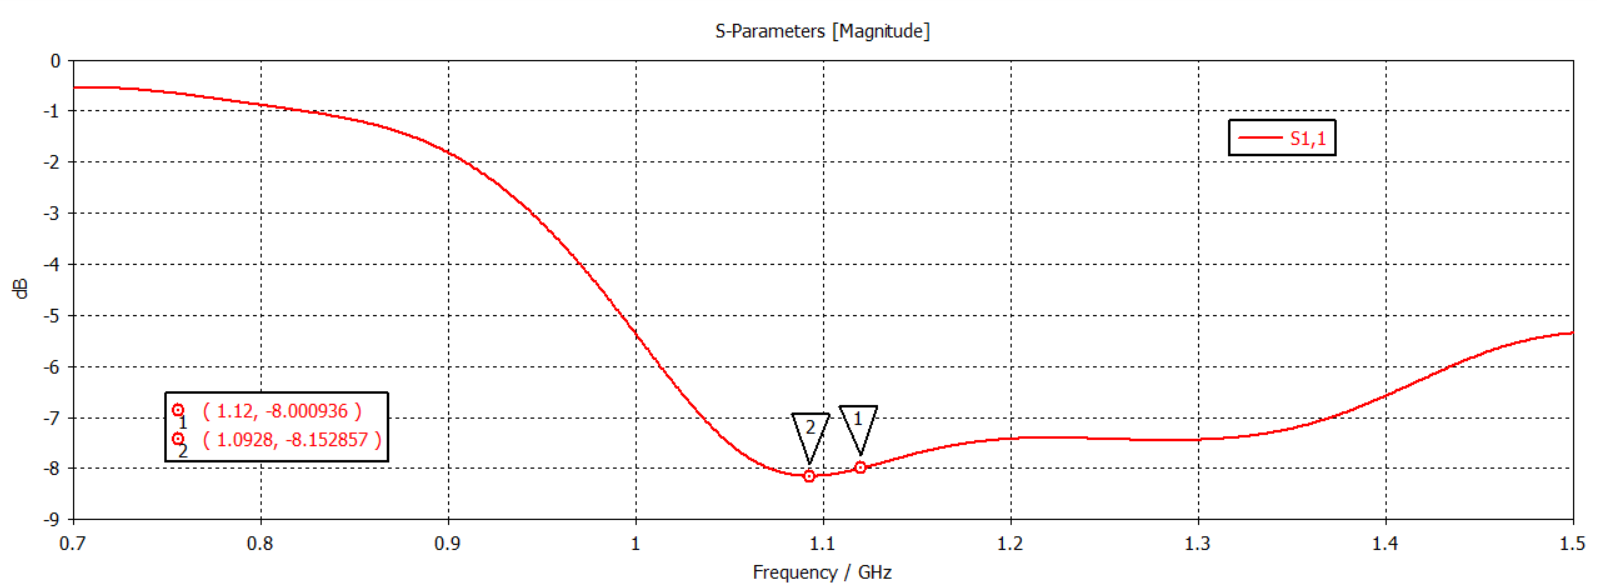
\includegraphics[width=0.82\textwidth]{figures/retuned/s11_body_5mm_retuned_L106p6_with_markers.png}
\caption{Return loss for the \(5~\mathrm{mm}\) body-separation case after retuning the dipole length to \(106.6~\mathrm{mm}\).}
\label{fig:retuned-l106p6-s11}
\end{figure}

\subsection{Additional Length-Tuning Iterations}

Additional length-tuning simulations were performed to determine whether further shortening could improve the match at \(1.120~\mathrm{GHz}\). Two additional lengths were tested:

\[
L = 105.8~\mathrm{mm}
\]

and

\[
L = 104.0~\mathrm{mm}.
\]

For the \(L=105.8~\mathrm{mm}\) case, CST showed

\[
f_{\min} = 1.1008~\mathrm{GHz},
\]

\[
S_{11,\min} = -7.970294~\mathrm{dB},
\]

and

\[
S_{11}(1.120~\mathrm{GHz}) = -7.904127~\mathrm{dB}.
\]

For the \(L=104.0~\mathrm{mm}\) case, the dominant matching minimum appeared at

\[
f_{\min} = 1.3208~\mathrm{GHz},
\]

with

\[
S_{11,\min} = -7.866346~\mathrm{dB}.
\]

At the target frequency,

\[
S_{11}(1.120~\mathrm{GHz}) = -7.569315~\mathrm{dB}.
\]

These additional simulations did not improve the return loss at the target frequency compared with the \(L=106.6~\mathrm{mm}\) case.

\begin{table}[htbp]
\centering
\caption{Length-tuning iterations for the \(5~\mathrm{mm}\) body-separation case.}
\label{tab:length-tuning-iterations}
\resizebox{\textwidth}{!}{%
\begin{tabular}{lcccc}
\hline
\textbf{Case} &
\(\boldsymbol{L}\) \textbf{(mm)} &
\textbf{Gap (mm)} &
\(\boldsymbol{f_{\min}}\) \textbf{(GHz)} &
\(\boldsymbol{S_{11}(1.120~GHz)}\) \textbf{(dB)} \\
\hline
Original body 5 mm & 122.0 & 2.0 & 0.9792 & -5.903831 \\
Retuned L106.6 & 106.6 & 2.0 & 1.0928 & -8.000936 \\
Retuned L105.8 & 105.8 & 2.0 & 1.1008 & -7.904127 \\
Retuned L104.0 & 104.0 & 2.0 & 1.3208 & -7.569315 \\
\hline
\end{tabular}%
}
\end{table}

The best length-only retuning result among the tested cases was obtained with

\[
L = 106.6~\mathrm{mm}.
\]

Although this case did not fully satisfy the \(-10~\mathrm{dB}\) matching criterion, it provided the best target-frequency return loss among the length-only retuned designs.

The return-loss response for the additional \(L=105.8~\mathrm{mm}\) tuning case is shown in Figure~\ref{fig:retuned-l105p8-s11}.

\begin{figure}[H]
\centering
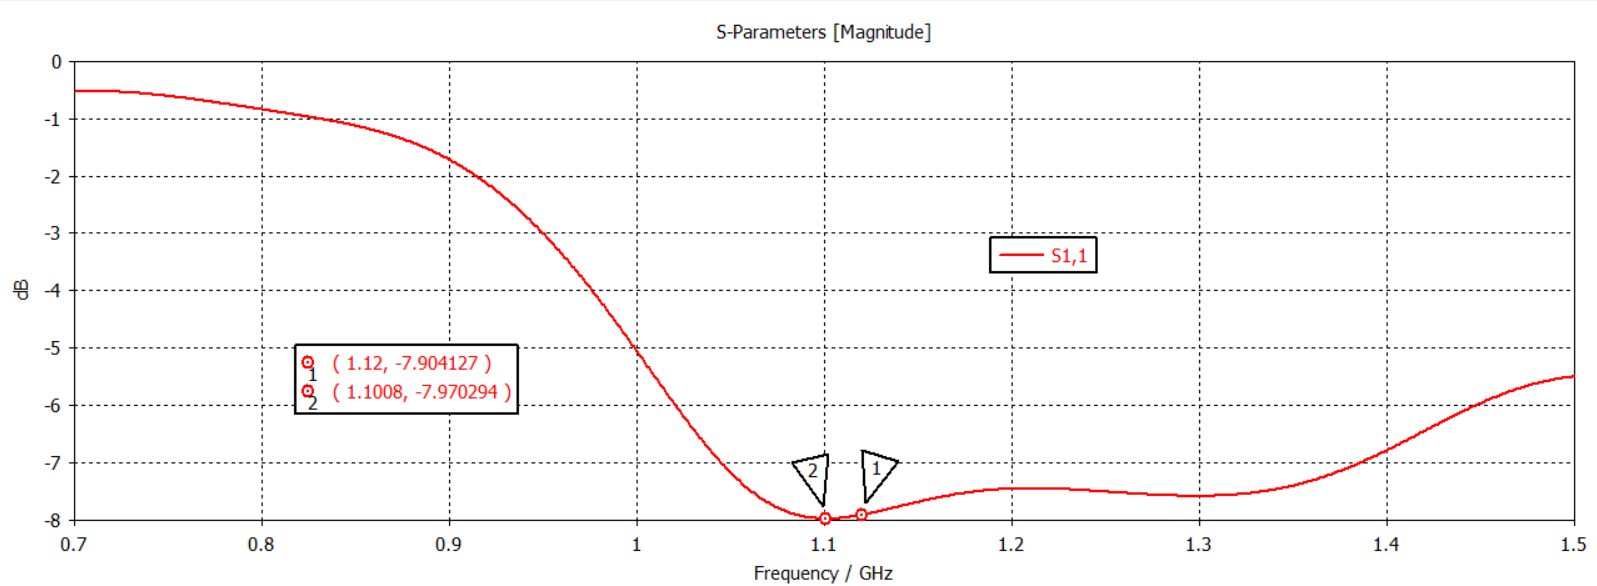
\includegraphics[width=0.82\textwidth]{figures/retuned/s11_body_5mm_retuned_L105p8_with_markers.png}
\caption{Return loss for the \(5~\mathrm{mm}\) body-separation case with retuned dipole length \(L=105.8~\mathrm{mm}\).}
\label{fig:retuned-l105p8-s11}
\end{figure}

The return-loss response for the shorter \(L=104.0~\mathrm{mm}\) tuning case is shown in Figure~\ref{fig:retuned-l104-s11}.

\begin{figure}[H]
\centering
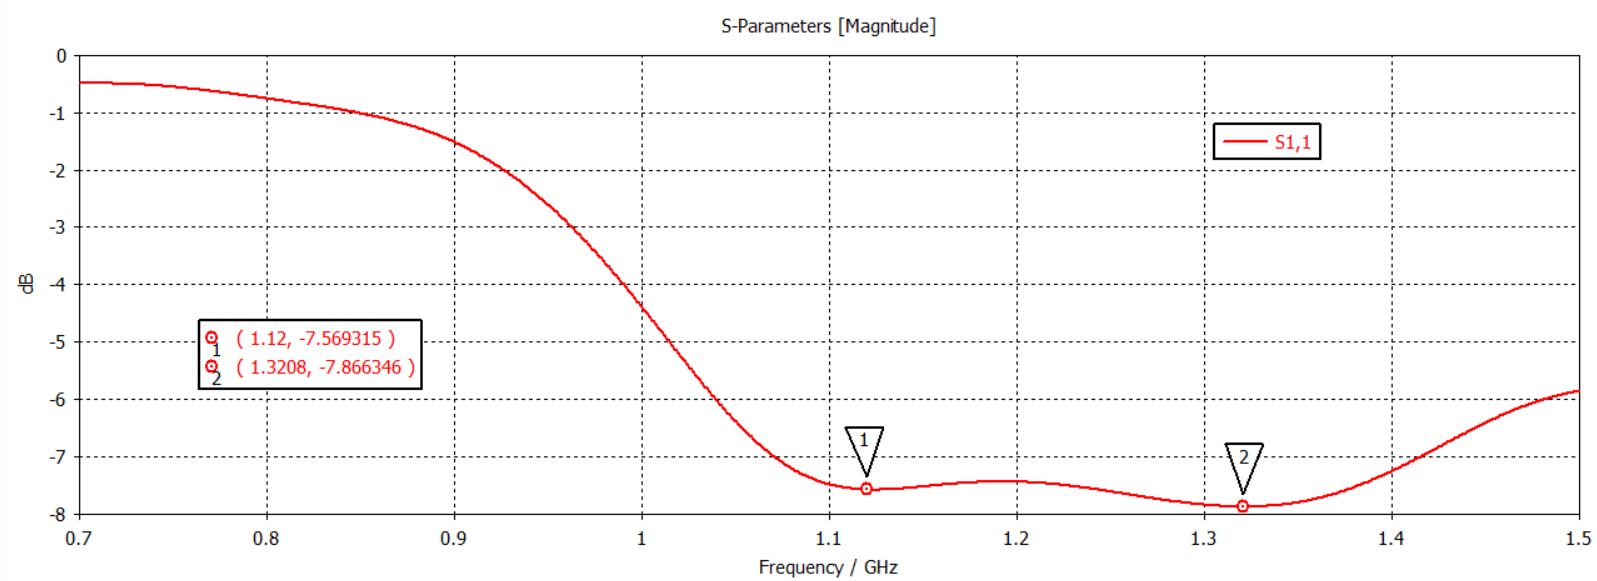
\includegraphics[width=0.82\textwidth]{figures/retuned/s11_body_5mm_retuned_L104_with_markers.png}
\caption{Return loss for the \(5~\mathrm{mm}\) body-separation case with retuned dipole length \(L=104.0~\mathrm{mm}\).}
\label{fig:retuned-l104-s11}
\end{figure}

\subsection{Feed-Gap Variation}

A feed-gap variation was also tested to examine whether changing the feed geometry could improve the impedance match. The dipole length was kept at

\[
L = 106.6~\mathrm{mm},
\]

but the feed gap was reduced from

\[
2.0~\mathrm{mm}
\]

to

\[
1.0~\mathrm{mm}.
\]

With a \(1.0~\mathrm{mm}\) feed gap, each arm length became

\[
L_{\mathrm{arm}}
=
\frac{106.6-1.0}{2}
=
52.8~\mathrm{mm}.
\]

The corresponding CST geometry is summarized in Table~\ref{tab:gap1-geometry}.

\begin{table}[htbp]
\centering
\caption{Retuned dipole geometry for \(L=106.6~\mathrm{mm}\) and \(1~\mathrm{mm}\) feed gap.}
\label{tab:gap1-geometry}
\begin{tabular}{lc}
\hline
\textbf{Parameter} & \textbf{Value} \\
\hline
Total dipole length & \(106.6~\mathrm{mm}\) \\
Feed gap & \(1.0~\mathrm{mm}\) \\
Wire radius & \(0.905~\mathrm{mm}\) \\
Each arm length & \(52.8~\mathrm{mm}\) \\
Right arm \(x\)-range & \(0.5~\mathrm{mm}\) to \(53.3~\mathrm{mm}\) \\
Left arm \(x\)-range & \(-53.3~\mathrm{mm}\) to \(-0.5~\mathrm{mm}\) \\
Port location & \(x=-0.5~\mathrm{mm}\) to \(x=0.5~\mathrm{mm}\) \\
Port reference impedance & \(50~\Omega\) \\
\hline
\end{tabular}
\end{table}

The CST result for the \(1~\mathrm{mm}\) gap case was

\[
f_{\min} = 1.0968~\mathrm{GHz},
\]

\[
S_{11,\min} = -7.925415~\mathrm{dB},
\]

and

\[
S_{11}(1.120~\mathrm{GHz}) = -7.821004~\mathrm{dB}.
\]

The far-field result at \(1.120~\mathrm{GHz}\) was

\[
\eta_{\mathrm{rad}} = -3.899~\mathrm{dB},
\]

\[
\eta_{\mathrm{tot}} = -4.683~\mathrm{dB},
\]

and

\[
G = 0.1812~\mathrm{dBi}.
\]

\begin{table}[htbp]
\centering
\caption{Feed-gap variation result for the \(5~\mathrm{mm}\) body-separation case.}
\label{tab:gap1-result}
\begin{tabular}{lc}
\hline
\textbf{Quantity} & \textbf{Value} \\
\hline
Dipole length & \(106.6~\mathrm{mm}\) \\
Feed gap & \(1.0~\mathrm{mm}\) \\
Minimum-\(S_{11}\) frequency & \(1.0968~\mathrm{GHz}\) \\
Minimum \(S_{11}\) & \(-7.925415~\mathrm{dB}\) \\
\(S_{11}\) at \(1.120~\mathrm{GHz}\) & \(-7.821004~\mathrm{dB}\) \\
Radiation efficiency at \(1.120~\mathrm{GHz}\) & \(-3.899~\mathrm{dB}\) \\
Total efficiency at \(1.120~\mathrm{GHz}\) & \(-4.683~\mathrm{dB}\) \\
Gain at \(1.120~\mathrm{GHz}\) & \(0.1812~\mathrm{dBi}\) \\
\hline
\end{tabular}
\end{table}

Although reducing the feed gap slightly moved the matching minimum, it did not improve the return loss at the target frequency compared with the \(L=106.6~\mathrm{mm}\), \(2~\mathrm{mm}\) gap case. Therefore, the \(1~\mathrm{mm}\) feed-gap case was not selected as the best retuned configuration.

The return-loss response for the \(L=106.6~\mathrm{mm}\), \(1~\mathrm{mm}\) feed-gap tuning case is shown in Figure~\ref{fig:retuned-l106p6-gap1-s11}.

\begin{figure}[htbp]
\centering
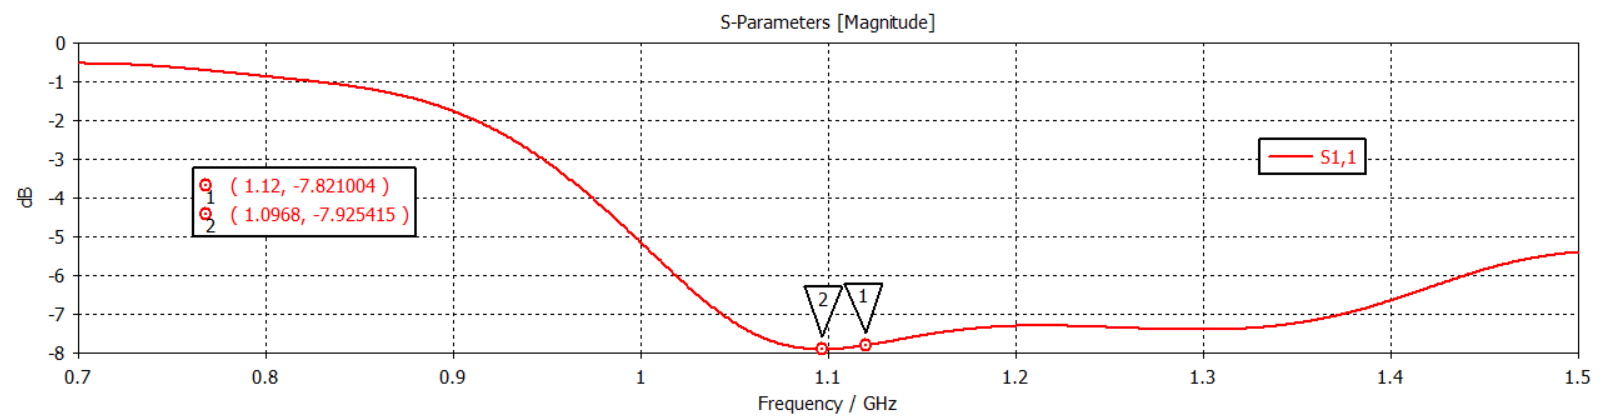
\includegraphics[width=0.82\textwidth]{figures/retuned/s11_body_5mm_retuned_L106p6_gap1_with_markers.png}
\caption{Return loss for the \(5~\mathrm{mm}\) body-separation case with \(L=106.6~\mathrm{mm}\) and \(1~\mathrm{mm}\) feed gap.}
\label{fig:retuned-l106p6-gap1-s11}
\end{figure}

The CST far-field parameter summary for the \(L=106.6~\mathrm{mm}\), \(1~\mathrm{mm}\) feed-gap tuning case is shown in Figure~\ref{fig:retuned-l106p6-gap1-farfield-parameters}.

\begin{figure}[H]
\centering
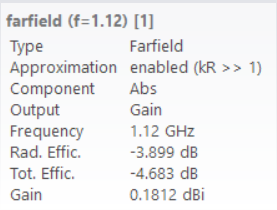
\includegraphics[width=0.42\textwidth]{figures/retuned/farfield_parameters_body_5mm_retuned_L106p6_gap1.png}
\caption{CST far-field parameter summary for the \(5~\mathrm{mm}\) body-separation case with \(L=106.6~\mathrm{mm}\) and \(1~\mathrm{mm}\) feed gap at \(1.120~\mathrm{GHz}\).}
\label{fig:retuned-l106p6-gap1-farfield-parameters}
\end{figure}

The three-dimensional gain pattern for the \(L=106.6~\mathrm{mm}\), \(1~\mathrm{mm}\) feed-gap tuning case is shown in Figure~\ref{fig:retuned-l106p6-gap1-3d-pattern}.

\begin{figure}[htbp]
\centering
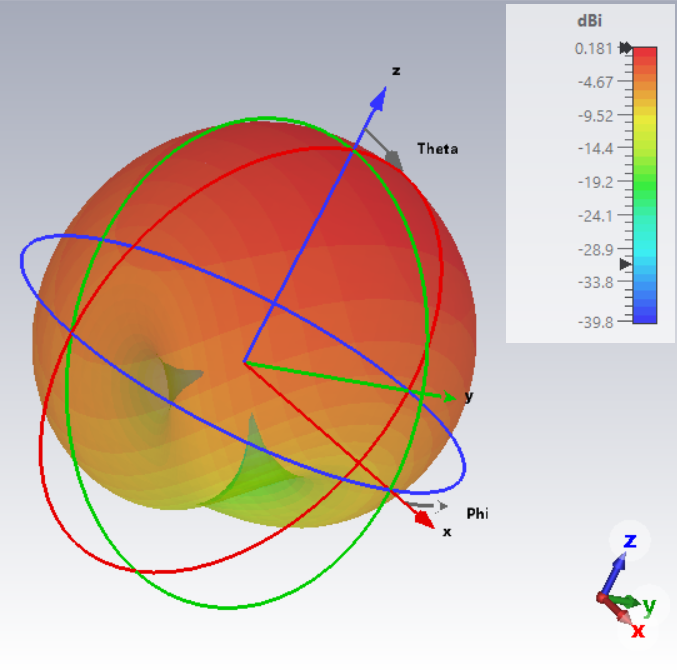
\includegraphics[width=0.82\textwidth]{figures/retuned/pattern_3d_gain_body_5mm_retuned_L106p6_gap1.png}
\caption{Three-dimensional gain pattern for the \(L=106.6~\mathrm{mm}\), \(1~\mathrm{mm}\) feed-gap case at \(1.120~\mathrm{GHz}\).}
\label{fig:retuned-l106p6-gap1-3d-pattern}
\end{figure}


\subsection{Retuning Summary}

The retuning results are summarized in Table~\ref{tab:retuning-summary}. The original \(5~\mathrm{mm}\) body case was poorly matched at the target frequency. Length-only retuning improved the target-frequency return loss, but it did not fully restore the \(-10~\mathrm{dB}\) matching condition.

\begin{table}[htbp]
\centering
\caption{Summary of retuning results for the \(5~\mathrm{mm}\) body-separation case.}
\label{tab:retuning-summary}
\resizebox{\textwidth}{!}{%
\begin{tabular}{lcccc}
\hline
\textbf{Case} &
\(\boldsymbol{L}\) \textbf{(mm)} &
\textbf{Gap (mm)} &
\(\boldsymbol{f_{\min}}\) \textbf{(GHz)} &
\(\boldsymbol{S_{11}(1.120~GHz)}\) \textbf{(dB)} \\
\hline
Original body 5 mm & 122.0 & 2.0 & 0.9792 & -5.903831 \\
Retuned L106.6 & 106.6 & 2.0 & 1.0928 & -8.000936 \\
Retuned L105.8 & 105.8 & 2.0 & 1.1008 & -7.904127 \\
Retuned L104.0 & 104.0 & 2.0 & 1.3208 & -7.569315 \\
Retuned L106.6 Gap1 & 106.6 & 1.0 & 1.0968 & -7.821004 \\
\hline
\end{tabular}%
}
\end{table}

The best tested retuned configuration was

\[
L = 106.6~\mathrm{mm},
\]

with a

\[
2.0~\mathrm{mm}
\]

feed gap. This configuration improved the return loss at the target frequency from

\[
-5.903831~\mathrm{dB}
\]

to

\[
-8.000936~\mathrm{dB}.
\]

However, the result remained above the desired \(-10~\mathrm{dB}\) threshold. This indicates that length-only retuning is not sufficient for complete impedance recovery near the lossy body model.

A more complete wearable antenna redesign would require additional techniques, such as adjusting the antenna height, modifying the conductor radius, changing the feed structure, using an impedance-matching network, adding an insulating spacer, or using a different wearable antenna geometry such as a planar or backed structure.
